\section{Simulation Budget}
\label{app-sec:compute-budget}


In simulation-based inference (SBI), an important consideration is the ability of a method to infer the posterior distribution under a restricted simulation budget.
The term \textit{simulation budget} typically refers to the number of allowed simulator evaluations — that is, the number of times the simulator is called to generate synthetic data.
Each simulator call produces a pair $(\boldsymbol{\theta}_i, \mathbf{y}_i)$, where $\mathbf{y}_i$ denotes the simulated observation corresponding to parameters $\boldsymbol{\theta}_i$.

Recently, with the advent of neural-based SBI methods, the simulation budget is often associated with the number of unique parameter–observation pairs used to train the neural density estimator.
In multi-round or active learning approaches, simulations from previous rounds can be reused for training, so the total number of simulator calls and the size of the training dataset are not necessarily identical.
Nevertheless, the number of unique simulations remains limited by the simulation budget, and neural estimators rely on these unique instances to learn an accurate posterior.


The simulation budget is an important consideration because it directly relates to computational cost. This arises for two main reasons: (a) each simulator call can be computationally expensive, and (b) training the neural density estimator on the resulting simulated dataset requires additional computation, which grows with dataset size. A common third cost is the time required to draw samples from the trained estimator; however, this cost is typically independent of the simulation budget and is therefore not counted here.
Therefore, simulation budget typically affects costs incured by (a) and/or (b).

For neural-based SBI methods, the simulation budget impacts both sources of computational cost: (a) the number of simulator calls and (b) the cost of training the neural density estimator. In contrast, for more traditional likelihood-free inference methods, such as approximate Bayesian computation (ABC), the simulation budget primarily affects (a), since these methods do not explicitly train a separate estimator.

Lately, modern computational frameworks, such as \texttt{JAX}, allow simulators to be implemented in a way that accelerates computation through vectorization. For example, a batch of parameters ${\boldsymbol{\theta}_i}$ for $i=1, \ldots, N$ can be evaluated on the same random seed $s$, producing outputs ${\mathbf{y}i}{i=1}^N$ at roughly the cost of a single simulator evaluation.
More generally, a grid of parameter–seed pairs ${\boldsymbol{\theta}_i, s_j}$ for $i = 1, \dots, N$ and $j = 1, \dots, S$ can also be computed efficiently, effectively generating $N \times S$ simulated pairs $(\boldsymbol{\theta}, \mathbf{y})$ at the cost of a `vectorized' evaluation, i.e., in significantly reduced computational overhead compared to $N \times S$ sequential evaluations.

These advancements can substantially reduce computational cost (a), as a single simulator call can now produce multiple $(\boldsymbol{\theta}, \mathbf{y})$ pairs through vectorized evaluation. However, they do not reduce cost (b), since training the neural density estimator still scales with the total number of simulated instances.
Therefore, although, this advancements benefits neural-based methods in terms of cost incured by (a), does not help them for (b).
This motivates the development of a method that avoids the computational cost of training an external neural estimator.

Therefore, we clarify that for \rromc, the term simulation budget is not directly applicable as a metric and, when we use it for comparison purposes, it refers to the number of independent calls to a vectorized simulator, where each call can produce multiple $(\boldsymbol{\theta}, \mathbf{y})$ pairs.
This definition emphasizes that for \rromc, the budget counts independent simulator evaluations rather than the total number of resulting dataset instances.

% However, as it becomes clear from runtime plots, it is indeed that case that a call to a vectorized simulator does nt 

\clearpage

\section{Methods}
\label{app-sec:methods}

Below, we provide information and the default hypeparameter setting that we use in the four methods we compare in the Introductory Example (Figure~\ref{fig:concept_example}) and the Mixture of Gaussians (MoG) benchmark~\ref{subsec:gaussian}.
% we compare \rromc~(our proposal) against three established neural-based methods—Neural Posterior Estimator~\citep[NPE,][]{greenberg2019automatic}, BayesFlow~\citep{radev2020bayesflow}, and Flow Matching Posterior Estimator~\citep[FMPE,][]{wildberger2023flow}.
% Below we provide 

\paragraph{R2OMC.}

A detailed description of the method can be found in Algorithm~\ref{alg:r2omc}. 

In Step 2 of Algorithm~\ref{alg:r2omc}, i.e., computing the uninformative dimensions, we typically use around 50 samples from the distribution \(p(u)\) and another 50 samples from \(p(\thb)\), with the parameter \(\tau\) set to machine precision, i.e., \(\tau \approx 0\). Similar results can be obtained with fewer samples, such as 10 or 20.

For Step 3, i.e., computing the optimal points \(\thb_{i,n}^*\), we use the Adam optimizer, with a learning rate between 0.01 and 0.2, depending on the specific problem. Our default choice is 0.01. The number of optimization steps varies between 50 and 400, with 50 as the default. The distance function \(d(\thb)\) is defined as the squared Euclidean distance between the simulator output and the observation, i.e., \(d(\thb) = \|\yb - \data_n\|^2_2\).
The number of seeds \(S\) used ranges from 100 to 10{,}000, with 1000 as the default.
The number of seeds corresponds to the simulation budget; for example, if a budget of 10,000 runs is available, we use (at most) 10,000 seeds.
Typically, we select 80\% of the seeds based on the best \(d_i^n(\thb_{i,n}^*)\).
However, the percentage of accepted seeds can vary between 50\% and 100\%, depending on the absolute values of \(d_i^n(\thb_{i,n}^*)\) for \(i = 1, \dots, S\).

For Step 5, i.e., constructing the hyperboxes, we use Algorithm~\ref{alg:region_construction}. We normally set \(\epsilon\) to be twice the distance of the `worst' accepted seed, i.e., \(\epsilon = 2 \max_i d_i^n(\thb_{i,n}^*)\), where \(i\) is an index over the accepted seeds. Alternatively, \(\epsilon\) can be set to a fixed value such as $0.1$. The typical settings for step size, number of steps, and refinements are \(\eta = 0.1\), \(L = 100\), and \(R = 1\), respectively.

For Step 7, i.e., sampling from the proposal distribution, we generate between 1000 and 100,000 candidate samples, with the default being 2000. From these candidates, we select 1000 via weighted sampling.
For computing the weights, $\{w_p\}_{p=1}^{P}$, we set $\epsilon$ to a value about twice the distance of the `worst' accepted seed, i.e., $\epsilon = 2 \max_{i,n} d_i^n(\thb_{i,n}^*)$. However, this can vary depending on the problem, and by testing different values.

% By default, we keep 1000 posterior samples, which are used to compute the \texttt{C2ST} score using another 1000 samples drawn from the true posterior.

\begin{algorithm}[!ht]
  \caption{Hyperbox Computation \newline
    \textit{Input:} Optimal point \(\thb^*\), distance function \(d(\thb)\), Jacobian \(\jac\) at \(\thb^*\) \newline
    \textit{Parameters:} Step size \(\eta\), number of refinements \(R\), number of steps \(L\), distance threshold \(\epsilon\)}
  \label{alg:region_construction}
  \begin{algorithmic}[1]
    \State Compute eigenvectors \(\vb_d\) of \(\jac^T\jac\) {\scriptsize (\(d = 1,\ldots,D)\)}
    \For{\(d = 1\) to \(D\)}
      \State Initialize endpoint \(\Tilde{\thb} \gets \thb^*\)
      \State Set refinement counter \(r \gets 0\)
      \Repeat{}
        \State Set step counter \(l \gets 0\)
        \Repeat{}
          \State Increment step counter \(l \gets l + 1\)
          \State Update \(\Tilde{\thb} \gets \Tilde{\thb} + \eta \vb_d\)
        \Until{\(d(\thb) > \epsilon\) or \(l = L\)}
        \State Move back one step \(\Tilde{\thb} \gets \Tilde{\thb} - \eta \vb_d\)
        \State Half the step size \(\eta \gets \eta/2\)
        \State Increment refinement counter \(r \gets r + 1\)
      \Until{\(r = R\)}
      \State Set \(\Tilde{\thb}\) as the endpoint
      \State Repeat steps 3-15 for \(\vb_d = - \vb_d\) and set \(\Tilde{\thb}\) as the negative endpoint
    \EndFor
    \State Define a uniform distribution \(q\) over the hyperbox
    \State \Return \(q\)
  \end{algorithmic}
\end{algorithm}


\paragraph{NPE}

For Neural Posterior Estimation (NPE), we use the variant denoted as \texttt{NPE\_C}~\citep{greenberg2019automatic} in the SBI benchmark~\citep{lueckmann2021benchmarking}.
\texttt{NPE\_C} estimates the posterior by training a neural network \( F(\mathbf{y}, \boldsymbol{\phi}) \) to approximate \( p(\boldsymbol{\theta} \mid \mathbf{y}) \) through a density estimator \( q_F(\mathbf{y}, \boldsymbol{\phi})(\boldsymbol{\theta}) \).
In the experiments, we use a neural spline flow as density estimator (\texttt{sbi.utils.get\_nn\_models.posterior\_nn()}).
The NPE configuration is summarized in Table~\ref{tab:npe_config}.

\begin{table}[h!]
\centering
\caption{Configuration of the Neural Posterior Estimation (NPE\_C) method.}
\label{tab:npe_config}
\begin{tabular}{lll}
\toprule
\textbf{Component} & \textbf{Parameter} & \textbf{Value} \\
\midrule
\multirow{5}{*}{\textbf{Density estimator} (\texttt{posterior\_nn})}
 & \texttt{model} & \texttt{'nsf'} \\
 & \texttt{hidden\_features} & 100 \\
 & \texttt{num\_transforms} & 8 \\
 & \texttt{num\_bins} & 10 \\
 & \texttt{z\_score\_x} & \texttt{'independent'} \\
 & \texttt{z\_score\_theta} & \texttt{'independent'} \\
\midrule
\multirow{3}{*}{\textbf{Training configuration} (\texttt{.train()})}
 & \texttt{training\_batch\_size} & 500 \\
 & \texttt{max\_num\_epochs} & 1000 \\
 & \texttt{force\_first\_round} & \texttt{True} \\
\bottomrule
\end{tabular}
\end{table}

\paragraph{BayesFlow.}

BayesFlow~\citep{radev2020bayesflow} is equivalent to Neural Posterior Estimation (NPE) with the key contribution of adding an
embedding network that automatically learns from the data appropriate summary statistics.
The \texttt{sbi} package provides access to these embeddings through the \texttt{sbi.neural\_nets.embedding\_nets()} interface.
In our experiments, we use the fully connected embedding network (\texttt{FCEmbedding}) and the default BayesFlow density estimator. 
The corresponding configurations are summarized in Table~\ref{tab:bayesflow_config}.

\begin{table}[h!]
\centering
\caption{Configuration of the BayesFlow embedding network and density estimator.}
\label{tab:bayesflow_config}
\begin{tabular}{lll}
\toprule
\textbf{Component} & \textbf{Parameter} & \textbf{Value} \\
\midrule
\multirow{3}{*}{\textbf{Embedding network} (\texttt{FCEmbedding})} 
 & \texttt{output\_dim} & 20 \\
 & \texttt{num\_layers} & 2 \\
 & \texttt{num\_hiddens} & 50 \\
\midrule
\multirow{5}{*}{\textbf{Density estimator} (\texttt{posterior\_nn})}
 & \texttt{model} & \texttt{'nsf'} \\
 & \texttt{hidden\_features} & 100 \\
 & \texttt{num\_transforms} & 8 \\
 & \texttt{z\_score\_x} & \texttt{'independent'} \\
 & \texttt{z\_score\_theta} & \texttt{'independent'} \\
\midrule
\multirow{3}{*}{\textbf{Training configuration} (\texttt{.train()})}
 & \texttt{training\_batch\_size} & 500 \\
 & \texttt{max\_num\_epochs} & 1000 \\
 & \texttt{force\_first\_round} & \texttt{True} \\
\bottomrule
\end{tabular}
\end{table}

\paragraph{FMPE.}

Flow Matching Posterior Estimation (FMPE)~\citep{{wildberger2023flow}} builds upon advances in generative modeling with continuous normalizing flows.
Similar in spirit to diffusion models, FMPE replaces discrete flow transformations with a continuous-time formulation based on flow matching.
In our experiments, we use the \texttt{sbi} implementation (\texttt{.FMPE()}) with a multilayer perceptron (\texttt{mlp}) as vector field estimator (\texttt{vf\_estimator}). The default configuration is summarized in Table~\ref{tab:fmpe_config}.

\begin{table}[h!]
\centering
\caption{Configuration of the Flow Matching Posterior Estimation (FMPE) method.}
\label{tab:fmpe_config}
\begin{tabular}{lll}
\toprule
\textbf{Component} & \textbf{Parameter} & \textbf{Value} \\
\midrule
\multirow{1}{*}{\textbf{Vector field estimator}}
 & \texttt{vf\_estimator} & \texttt{'mlp'} \\
\midrule
\multirow{3}{*}{\textbf{Training configuration} (\texttt{.train()})}
 & \texttt{training\_batch\_size} & 500 \\
 & \texttt{max\_num\_epochs} & 1000 \\
 & \texttt{force\_first\_round\_loss} & \texttt{True} \\
\bottomrule
\end{tabular}
\end{table}


\clearpage


  
\section{Introductory Example}
\label{app-sec:intro-example}

\subsection{Problem Definition}

We provide further details on the introductory example of Figure~\ref{fig:concept_example}.  
The example comes with three variants, that we refer to as: (1) \textbf{Simple}, (2) \textbf{High-dimensional}, and (3) \textbf{Distractors}.
%
Simple (1) and High-dimensional (2) share the same setup.
Between them, the only difference is the parameter dimension $D$ and the output dimension $D_y$ which are: $D=D_y=2$ in (1) and $D=D_y=10$ in (2).

In both (1) and (2), the simulator is:
\begin{equation}
  \label{eq:intro-simulator}
  \yb \sim \frac{1}{2} \sum_{s \in \{+1, -1\}} \mathcal{N}(\thb + s\boldsymbol{\mu}, \sigma^2 \mathbf{I}), 
  \quad \boldsymbol{\mu} = \mathbf{1}, \ \sigma = 0.2.
\end{equation}

In the Distractors (3) variant, the parameter space is $D = 2$, but we add $D_{\text{dist}} = 18$ distractor dimensions to the output, yielding $D_y = 20$.
Thus, in (3), the simulator becomes:

\begin{equation}
  \label{eq:intro-simulator-distractor}
  \yb = (\mathbf{y}^{(1)}, \mathbf{y}^{(2)}), \quad
  \mathbf{y}^{(1)} \sim \frac{1}{2} \sum_{s \in \{+1, -1\}} \mathcal{N}(\thb + s\boldsymbol{\mu}, \sigma^2 \mathbf{I}), \quad
  \mathbf{y}^{(2)} \sim \mathcal{U}(-\mathbf{3}, \mathbf{3}),
\end{equation}
where $\boldsymbol{\mu} = \mathbf{1}$ and $\sigma=0.2$.  
%
For all variants, the prior is $\mathcal{U}(-\mathbf{3}, \mathbf{3})$ and the observation is $\data = \mathbf{0} \in \mathbb{R}^{D_y}$.

\subsection{Ground Truth Posterior}

\paragraph{Simple and High-dimensional Case.}

The posterior is given by
\begin{align}
  p(\thb \mid \data) &\propto p(\thb) p(\data \mid \boldsymbol{\theta}) \\
  &\propto p(\thb) \left[ \mathcal{N}(\data; \boldsymbol{\theta} - \boldsymbol{\mu}, \sigma^2\mathbf{I}) + \mathcal{N}(\data; \boldsymbol{\theta} + \boldsymbol{\mu}, \sigma^2\mathbf{I}) \right] \label{eq:intro-simple-1} \\
  &\propto p(\thb) \left[ \mathcal{N}(\boldsymbol{\theta}; \boldsymbol{\mu}, \sigma^2\mathbf{I}) + \mathcal{N}(\boldsymbol{\theta}; -\boldsymbol{\mu}, \sigma^2\mathbf{I}) \right] \label{eq:intro-simple-2} \\
  &\propto
    \begin{cases}
      \mathcal{N}(\boldsymbol{\theta}; \boldsymbol{\mu}, \sigma^2\mathbf{I}) + \mathcal{N}(\boldsymbol{\theta}; -\boldsymbol{\mu}, \sigma^2\mathbf{I}), & \boldsymbol{\theta} \in [-3, 3]^D, \\
      0, & \text{otherwise}.
    \end{cases}
    \label{eq:intro-simple}
\end{align}

From~(\ref{eq:intro-simple-1}) to~(\ref{eq:intro-simple-2}), we use the property: $\mathcal{N}(\yb; \thb - \boldsymbol{\mu}, \Sigma) = \mathcal{N}(\thb; \yb + \boldsymbol{\mu} , \Sigma)$.

\paragraph{Distractors Case.}

In the distractors variant, the posterior over $\boldsymbol{\theta}$ remains unchanged.  
Formally:
\begin{align}
  p(\boldsymbol{\theta} \mid \data)
  &\propto p(\boldsymbol{\theta}) p(\data \mid \boldsymbol{\theta}) \\
  &\propto p(\boldsymbol{\theta}) p((\mathbf{y}^{o,(1)}, \mathbf{y}^{o,(2)}) \mid \boldsymbol{\theta}) \label{eq:intro-distractors-1} \\
  &\propto p(\boldsymbol{\theta}) \, p(\mathbf{y}^{o,(1)} \mid \boldsymbol{\theta}) \, p(\mathbf{y}^{o,(2)} \mid \boldsymbol{\theta}) \label{eq:intro-distractors-2} \\
  &\propto p(\boldsymbol{\theta}) \, p(\mathbf{y}^{o,(1)} \mid \boldsymbol{\theta}) \, p(\mathbf{y}^{o,(2)}) \label{eq:intro-distractors-3} \\
  &\propto
    \begin{cases}
      \mathcal{N}(\boldsymbol{\theta}; \boldsymbol{\mu}, \sigma^2\mathbf{I}) + \mathcal{N}(\boldsymbol{\theta}; -\boldsymbol{\mu}, \sigma^2\mathbf{I}), & \boldsymbol{\theta} \in [-3, 3]^D, \\
      0, & \text{otherwise}.
    \end{cases}
  \label{eq:intro-distractors}
\end{align}

Steps (\ref{eq:intro-distractors-1}) to (\ref{eq:intro-distractors-2}) use independence between $\mathbf{y}^{o,(1)}$ and $\mathbf{y}^{o,(2)}$, and steps (\ref{eq:intro-distractors-2}) to (\ref{eq:intro-distractors-3}) use that $\mathbf{y}^{o,(2)}$ is independent of $\thb$.

\subsection{Experimental Setup and Hyperparameter Configuration}

All methods were evaluated for simulation budgets of
$
[1{,}000, 10{,}000, 30{,}000, 40{,}000, 50{,}000]
$.
For each method, we drew 1{,}000 samples from the approximate posterior and compared them against 1{,}000 ground-truth samples using the C2ST score.  
Each experiment was repeated across 5 independent random seeds, so we report the average C2ST scores among the independent runs.

The experiment goal is to analyze the performance of each method in two regimes.
The \textbf{low-budget/low-runtime} regime, where the budget is always $1{,}000$ and the
\textbf{high-budget/high-runtime} regime, where the budget is between $10{,}000$ and $50{,}000$.
In the low-runtime regime, we simply report the mean C2ST score and runtime for a budget of $1{,}000$.  
In the high-runtime regime, we select the minimum budget that achieves an average C2ST below 0.65. If no budget meets this threshold, we select the budget with the lowest C2ST (which is always 50{,}000 in this case).
We report the mean C2ST and runtime of the selected budget

Below, we detail the hyperparameter configuration for each method, highlighting the deviations from the default settings.

\paragraph{ROMC} 
For \rromc, we used at most a maximum of $S = 1{,}000$ seeds, corresponding to roughly 1{,}000 independent simulator calls, as this budget was enough for a near-optimal C2ST score.
The modified fitting parameters are: \texttt{\{"pcg\_to\_keep":1.\}}, i.e., we keep all optimization ending points $\{\thb_i^*\}_{i=1}^{S}$.

\paragraph{NPE-C} 
The modified fitting parameters are:
\texttt{\{"batch\_size":100, "training\_batch\_size":100\}}

\paragraph{BayesFlow} 
The modified fitting parameters are: \texttt{\{"embedding\_net\_output\_dim": 2\}} for the Simple and Distractor variants, and \texttt{10} for the High-dimensional variant.

\paragraph{Flow-Matching} All arguments were default.

\subsection{Conclusions}

Figure~\ref{fig:concept_example} illustrates the key-findings presented below.

In the simple scenario (1), most methods perform well across both low- and high-budget regimes. Only FMPE requires a substantial simulation budget and runtime to succeed, whereas the remaining methods already achieve good performance under low-budget conditions.

However, the picture changes as the task becomes more challenging—either through the addition of distractors (2) or by increasing dimensionality (3). In these settings, all neural-based methods fail to perform adequately with a low simulation budget and require significantly higher budgets, and consequently higher runtimes, to succeed. BayesFlow, in particular, fails to converge even under the high-budget regime. In contrast, \rromc~achieves competitive performance using only 1,000 simulations, resulting in substantially lower runtime requirements.

Overall, the results highlight an important trend: as dimensionality increases or distractor dimensions are introduced, neural-based methods demand increasingly larger simulation budgets to achieve reliable performance. While a budget of 50,000 simulations is not prohibitive—modern infrastructure can handle even 100,000 simulations within reasonable runtimes—the observed trend is clear. With increases in dimensionality, additional distractors, or more complex simulators (beyond simple Gaussian noise), the required number of simulations grows rapidly. Consequently, under strict budget and runtime constraints, these neural-based approaches are likely to face significant limitations.

\clearpage
\section{Experiments: Additional Information}
\label{app-sec:experiments}

We here provide some additional information on the experiments presented in the main text.

\subsection{Mixture of Gaussians (MoG) Benchmark}

The Mixture of Gaussians (MoG) benchmark evaluates how simulation-based inference (SBI) methods scale with increasing problem dimensionality.
Specifically, it assesses whether higher-dimensional problems require larger simulation budgets to achieve accurate inference, i.e., whether there exists a correlation between dimensionality and the required number of simulations.

To this end, we consider four simulator variants:
$S_{\texttt{base}}$ (1), $S_{\texttt{base}}^{\texttt{dist}}$ (2), $S_{\texttt{MoG}}$ (3), and $S_{\texttt{MoG}}^{\texttt{dist}}$ (4).
Each simulator is tested across different dimensionalities, $D = {2, 5, 10, 15, 20}$.
For each configuration, we evaluate every method’s performance across multiple simulation budgets using the C2ST metric.

\subsubsection{Problem definition and ground truth posterior}

\textbf{Base simulator - without distractors (1):}

\begin{tabular}{@{}ll@{}}
  \textbf{Prior} & $\thb \sim \mathcal{U}(-\mathbf{3}, \mathbf{3})$ \\ [5pt]
  \textbf{Simulator} & $\yb \sim \mathcal{N}(\thb + \boldsymbol{\mu}, \sigma^2 \mathbf{I}) \label{eq:mog_base}$, with $\boldsymbol{\mu} = \mathbf{1}, \sigma^2 = 0.2^2$ \\ [5pt]
  \textbf{Dimensionality} & $\thb \in \mathbb{R}^{D}$, $\yb \in \mathbb{R}^{D}$ \\ [5pt]
  \textbf{Observation} & $\data = (0, \ldots, 0)$ where $\data \in \mathbb{R}^D$ \\ [5pt]
  \textbf{Posterior} & $ p(\thb | \data) \propto
                                    \begin{cases}
                                      \mathcal{N}(\thb; -\boldsymbol{\mu}, \sigma^2 \mathbf{I}), & \text{if } \thb \in [-3, 3]^D, \\
                                      0, & \text{otherwise}.
                                    \end{cases} $ \\ [5pt]
\end{tabular}

\textbf{Proof of the posterior:}
%
\begin{align}
  p(\thb | \data) &\propto p(\thb) p(\data | \thb) \label{eq:mog_base_posterior-1} \\
                  &\propto p(\thb) \mathcal{N}(\data; \thb + \boldsymbol{\mu}, \sigma^2 \mathbf{I}) \label{eq:mog_base_posterior-2} \\
                  &\propto p(\thb) \mathcal{N}(\thb; \data - \boldsymbol{\mu}, \sigma^2 \mathbf{I}) \label{eq:mog_base_posterior-3} \\
                  &\propto
                    \begin{cases}
                      \mathcal{N}(\thb; - \boldsymbol{\mu}, \sigma^2 \mathbf{I}), & \text{if } \thb \in [-3, 3]^D, \\
                      0, & \text{otherwise}.
                    \end{cases} \label{eq:mog_base_posterior}
\end{align}

From~(\ref{eq:mog_base_posterior-2}) to~(\ref{eq:mog_base_posterior-3}), we apply the property: $\mathcal{N}(\yb; \thb + \boldsymbol{\mu}, \Sigma) = \mathcal{N}(\thb; \yb - \boldsymbol{\mu} , \Sigma)$.


\textbf{Base simulator - with distractors (2):}

\begin{tabular}{@{}ll@{}}
  \textbf{Prior} & $\thb \sim \mathcal{U}(-\mathbf{3}, \mathbf{3})$ \\ [5pt]
  \textbf{Simulator} & $\yb = (\mathbf{y^{(1)}}, \mathbf{y^{(2)}})$, \\ [5pt]
  & $\mathbf{y^{(1)}} \sim \mathcal{N}(\thb + \boldsymbol{\mu}, \sigma^2 \mathbf{I})$, $\boldsymbol{\mu} = \mathbf{1}$, $\sigma^2=0.2^2$, \\ [5pt]
  & $\mathbf{y^{(2)}} \sim \mathcal{U}(\mathbf{-3}, \mathbf{3})$ \\ [5pt]
  \textbf{Dimensionality} & $\thb \in \mathbb{R}^D,  \yb \in \mathbb{R}^{D + 18}$, $\yb^{(1)} \in \mathbb{R}^{D}$, $\yb^{(2)} \in \mathbb{R}^{18}$\\ [5pt]
  \textbf{Observation} & $\data = (\mathbf{y^{o, (1)}}, \mathbf{y^{o, (2)}})$, where both $\mathbf{y^{o, (1)}}$ and $\mathbf{y^{o, (2)}}$  are $(0, \ldots, 0) $ \\ [5pt]
  \textbf{Posterior} & $ p(\thb | \data) \propto
                                    \begin{cases}
                                      \mathcal{N}(\thb; -\boldsymbol{\mu}, \sigma^2 \mathbf{I}), & \text{if } \thb \in [-3, 3]^D, \\
                                      0, & \text{otherwise}.
                                    \end{cases} $ \\ [5pt]
\end{tabular}

The ground truth posterior is the same as in~(\ref{eq:mog_base_posterior}), as the distractors do not affect the posterior, see (\ref{eq:intro-distractors}).

\textbf{MoG simulator - without distractors (3):}

\begin{tabular}{@{}ll@{}}
  \textbf{Prior} & $\thb \sim \mathcal{U}(-\mathbf{3}, \mathbf{3})$ \\ [5pt]
  \textbf{Simulator} & $\yb \sim \frac{1}{2} \sum_{s \in \{-1, +1\}} \mathcal{N}(\thb + s\boldsymbol{\mu}, \sigma^2\mathbf{I})$, $\boldsymbol{\mu} = \mathbf{1}$ and $\sigma^2=0.2^2$ \\ [5pt]
  \textbf{Dimensionality} & $\thb \in \mathbb{R}^{D}$, $\yb \in \mathbb{R}^{D}$ \\ [5pt]
  \textbf{Observation} & $\data = (0, \ldots, 0)$ where $\data \in \mathbb{R}^D$ \\ [5pt]
  \textbf{Posterior} & $ p(\thb | \data) \propto
                                    \begin{cases}
                                      \mathcal{N}(\thb; \sum_{s \in \{-1, +1\}} \mathcal{N}(s\boldsymbol{\mu}, \sigma^2 \mathbf{I}), & \text{if } \thb \in [-3, 3]^D, \\
                                      0, & \text{otherwise}.
                                    \end{cases} $ \\ [5pt]
\end{tabular}

The MoG simulator is the same as in the introductory example, so the proof is equivalent to Section~\ref{app-sec:intro-example}.

\textbf{MoG simulator - with distractors (4):}

\begin{tabular}{@{}ll@{}}
  \textbf{Prior} & $\thb \sim \mathcal{U}(-\mathbf{3}, \mathbf{3})$ \\ [5pt]
  \textbf{Simulator} & $\yb=(\mathbf{y^{(1)}}, \mathbf{y^{(2)}})$,\\[5pt]
  &$\mathbf{y^{(1)}} \sim \frac{1}{2} \sum_{s \in \{-1, +1\}} \mathcal{N}(\thb + s\boldsymbol{\mu}, \sigma^2\mathbf{I})$, $\boldsymbol{\mu} = \mathbf{1}$ and $\sigma^2=0.2^2$ \\[5pt]
  &$\mathbf{y^{(2)}} \sim \mathcal{U}(\mathbf{-3}, \mathbf{3})$ \\ [5pt]
  \textbf{Dimensionality} & $\thb \in \mathbb{R}^{D}$, $\yb \in \mathbb{R}^{D + 18}$, $\yb^{(1)} \in \mathbb{R}^{D}$, $\yb^{(2)} \in \mathbb{R}^{18}$ \\ [5pt]
  \textbf{Observation} & $\data = (\mathbf{y^{o, (1)}}, \mathbf{y^{o, (2)}})$, where both $\mathbf{y^{o, (1)}}$ and $\mathbf{y^{o, (2)}}$  are $(0, \ldots, 0) $ \\ [5pt]
  \textbf{Posterior} & $ p(\thb | \data) \propto
                       \begin{cases}
                         \mathcal{N}(\thb; \sum_{s \in \{-1, +1\}} \mathcal{N}(s\boldsymbol{\mu}, \sigma^2 \mathbf{I}), & \text{if } \thb \in [-3, 3]^D, \\
                                      0, & \text{otherwise}.
                                    \end{cases} $ \\ [5pt]
\end{tabular}

The MoG simulator is the same as in the introductory example, so the proof is equivalent to Section~\ref{app-sec:intro-example}.

\subsubsection{Experimental Setup and Hyperparameter Configuration}

For each of the four problems (1)--(4) and across all dimensionalities 
$D \in \{2, 5, 10, 15, 20\}$, we evaluated all methods under simulation budgets of
\(
[1{,}000, 5{,}000, 10{,}000, 50{,}000, 100{,}000],
\)
recording both the C2ST score and the runtime.

To reduce experimental cost, we adopted an early-stopping criterion: if a method achieved a C2ST score below 0.75 for a given dimensionality $D$ at a certain budget, we did not evaluate it at higher budgets. Each experiment was repeated with three independent random seeds, and we report the average C2ST scores across these runs.
For each method, we drew 1{,}000 samples from the approximate posterior and compared them against 1{,}000 ground-truth samples using the C2ST metric.

The goal of this experiment is to assess whether the required simulation budget---and consequently, the runtime---increase with problem dimensionality. To this end, we identify the minimum budget at which each method achieves successful inference, defined as an average C2ST score below 0.75. We report both the mean C2ST and mean runtime across the three runs.

Below, we detail the hyperparameter configuration for each method, emphasizing deviations from the default settings.

\paragraph{ROMC} 
For \rromc, we used at most a maximum of $S = 1{,}000$ seeds, corresponding to roughly 1{,}000 independent simulator calls, as this budget was enough for a near-optimal C2ST score.
The modified fitting parameters are: \texttt{\{"pcg\_to\_keep":1., "epochs": 10, "alpha": 0.1\}} and the modified sampling parameters are: \texttt{\{"samples\_per\_region": 2\}}.

\paragraph{NPE-C} 
The modified fitting parameters are:
\texttt{\{"num\_transforms":16, "num\_bins":16 "hidden\_features":200, "training\_batch\_size": 500\}}

\paragraph{BayesFlow} 

The modified fitting parameters are:
\texttt{\{
  "batch\_size": 500,
  "training\_batch\_size": 500,
  "embedding\_net\_num\_layers": 2,
  "embedding\_net\_num\_hiddens": 32
  \}}.
Finally, the parameter
\texttt{\{"embedding\_net\_output\_dim": dim\}} is for the non-distractor variants ((1), (3)) and \texttt{dim + 18} for the distractor variants ((2), (4)).

\paragraph{Flow-Matching}
The modified fitting parameters are:
\texttt{\{"batch\_size": 100, "training\_batch\_size": 100\}}.

\subsubsection{Results}

Figure~\ref{fig:high_dim_benchmark} in the main paper summarizes the results using success frontier plots, which depict the minimum runtime required to achieve successful inference across different dimensions $D$. 
Inference is deemed successful when the mean \CtwoST~score is less than or equal to 0.75. 
The corresponding plots using the simulation budget (instead of runtime) are shown in Figure~\ref{fig:mog_benchmark_frontier_budget}. 
This figure complements Figure~\ref{fig:high_dim_benchmark} validating that the factor that incurs longer runtimes is the increased simulation budget required at higher dimensionalities.

For a more detailed view, Figures~%
\ref{fig:mog_benchmark_base_heatmaps} ($\mathcal{S}_{\mathtt{base}}$), 
\ref{fig:mog_benchmark_base_distractors_heatmaps} ($\mathcal{S}_{\mathtt{base}}^{\mathtt{dist}}$), 
\ref{fig:mog_benchmark_mog_heatmaps} ($\mathcal{S}_{\mathtt{MoG}}$), and 
\ref{fig:mog_benchmark_mog_distractors_heatmaps} ($\mathcal{S}_{\mathtt{MoG}}^{\mathtt{dist}}$) 
report the mean \CtwoST~score for each method across all dimensionalities and budgets.

All neural-based methods exhibit a consistent trend: as $D$ increases, the simulation budget required for accurate posterior inference grows rapidly, often exceeding $100{,}000$ simulations and resulting in runtimes that often exceed one hour. 
Runtimes increase more sharply for $S_{\mathtt{MoG}}$ compared to $S_{\mathtt{base}}$, and are higher in the distractor settings than in the simpler ones. 

In contrast, \rromc~achieves successful inference within a few seconds across all dimensionalities and simulator configurations.


\begin{figure*}[!t]
  \centering
  \begin{subfigure}[b]{0.245\textwidth}
    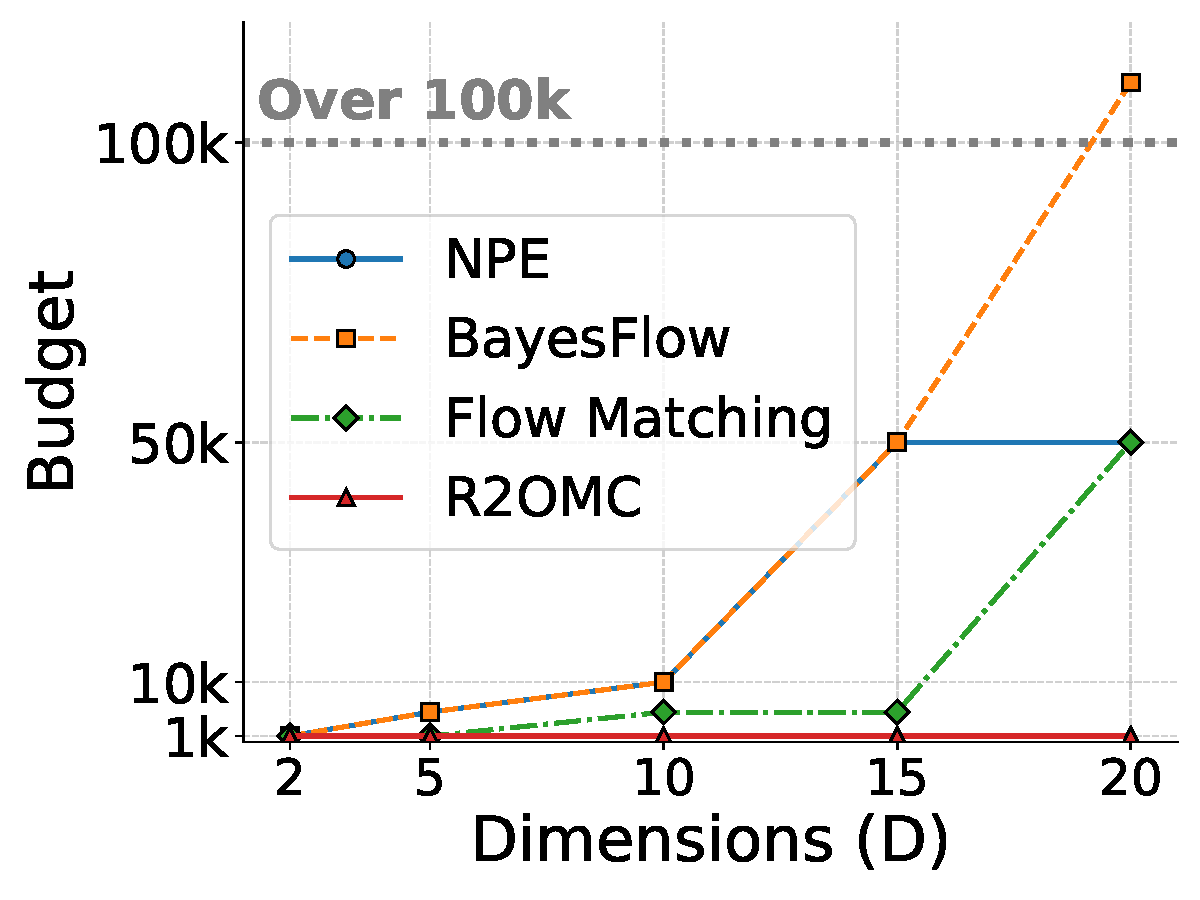
\includegraphics[width=\linewidth]{./figures/mog_benchmark/single_mode/c2st_frontier}
    \caption{$S_{\mathtt{base}}$}
  \end{subfigure}
  \begin{subfigure}[b]{0.245\textwidth}
    
\includegraphics[width=\linewidth]{./figures/mog_benchmark/single_mode_distractors/c2st_frontier}
    \caption{$S_{\mathtt{base}}^{\mathtt{dist}}$}
  \end{subfigure}
  \begin{subfigure}[b]{0.245\textwidth}
    
\includegraphics[width=\linewidth]{./figures/mog_benchmark/two_modes/c2st_frontier}
    \caption{$S_{\mathtt{MoG}}$}
  \end{subfigure}
  \begin{subfigure}[b]{0.245\textwidth}
    
\includegraphics[width=\linewidth]{./figures/mog_benchmark/two_modes_distractors/c2st_frontier}
    \caption{$S^{\mathtt{dist}}_{\mathtt{MoG}}$}
  \end{subfigure}
  \caption{MoG benchmark: Success Frontier plots showing the lowest budget required to reach a C2ST score $\leq 0.75$ for varying $D$.}
  \label{fig:mog_benchmark_frontier_budget}
\end{figure*}

\begin{figure}
    \centering
    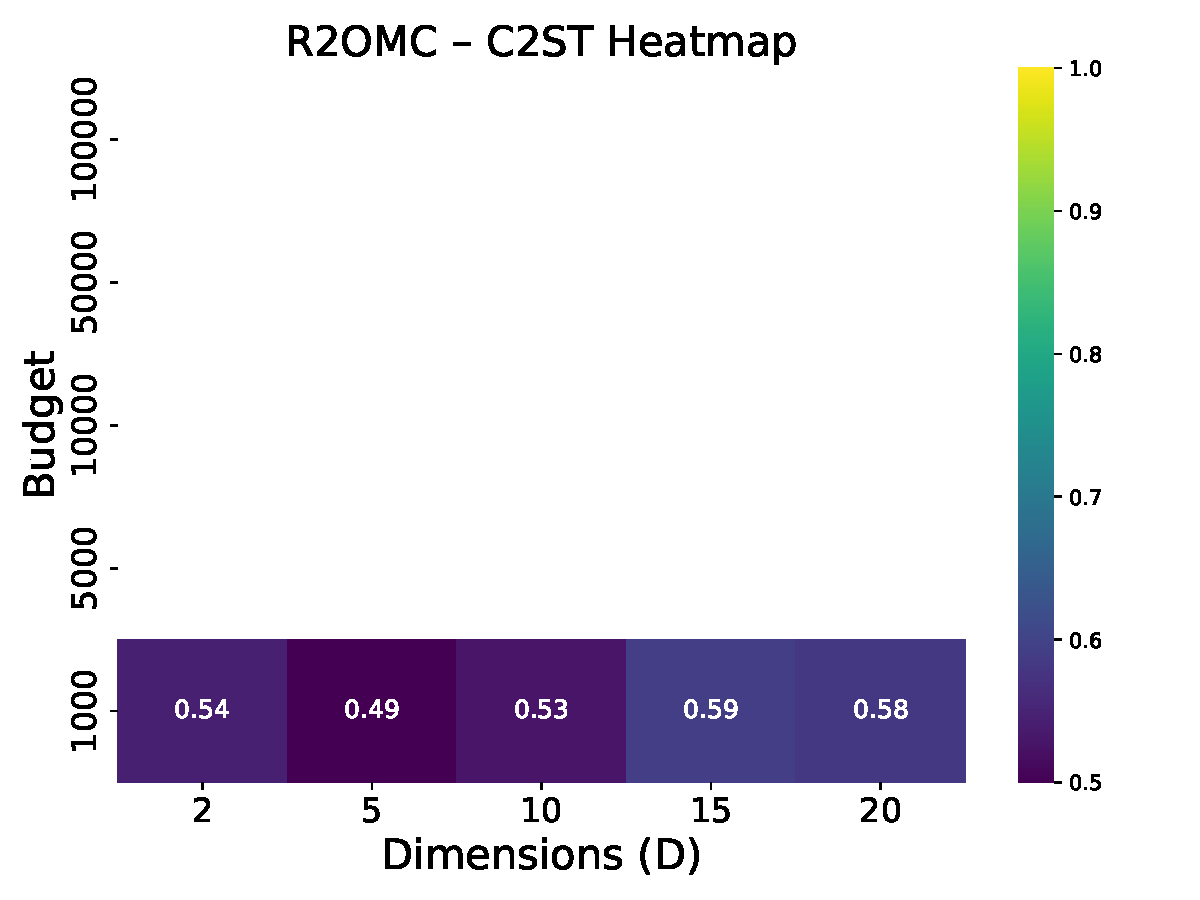
\includegraphics[width=.24\linewidth]{figures/mog_benchmark/single_mode/R2OMC_c2st_heatmap}
    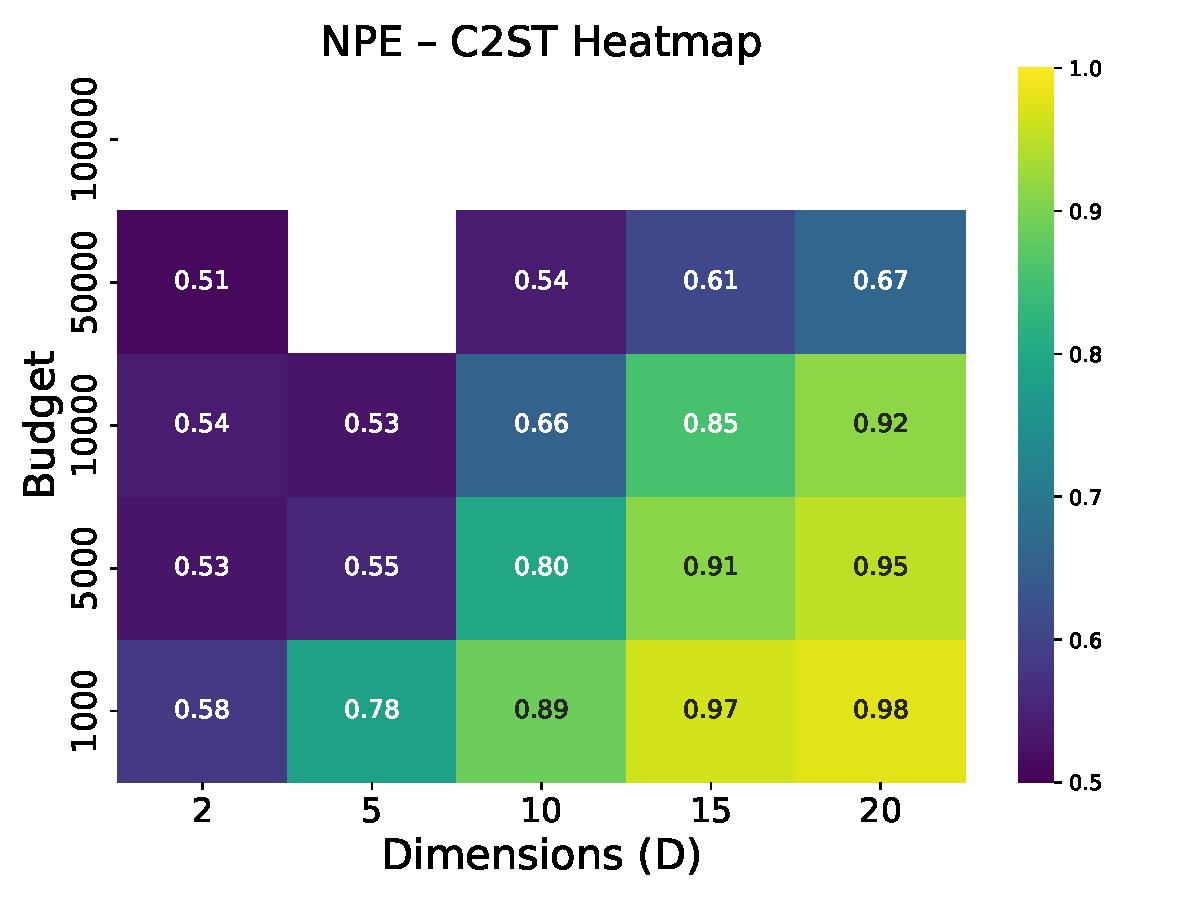
\includegraphics[width=.24\linewidth]{figures/mog_benchmark/single_mode/NPE_c2st_heatmap}
    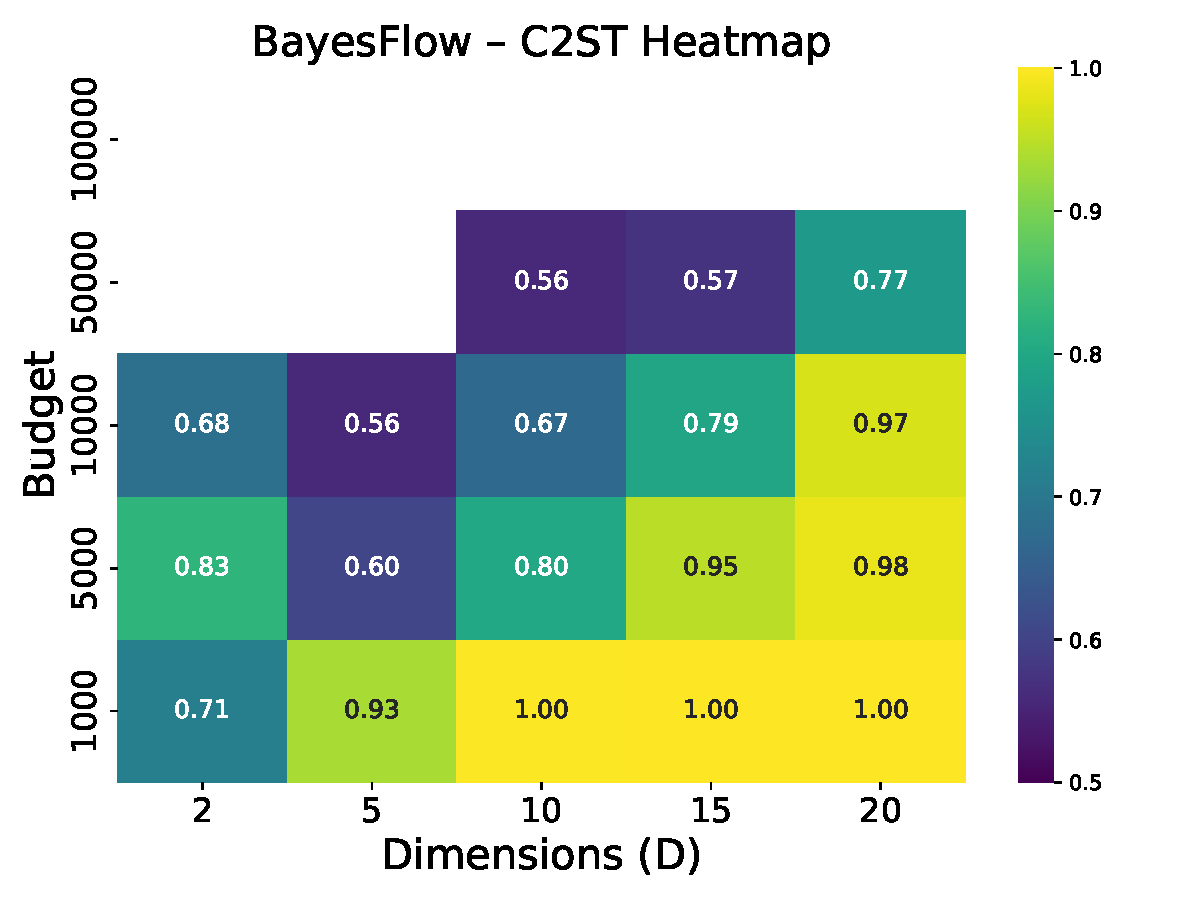
\includegraphics[width=.24\linewidth]{figures/mog_benchmark/single_mode/BayesFlow_c2st_heatmap}
    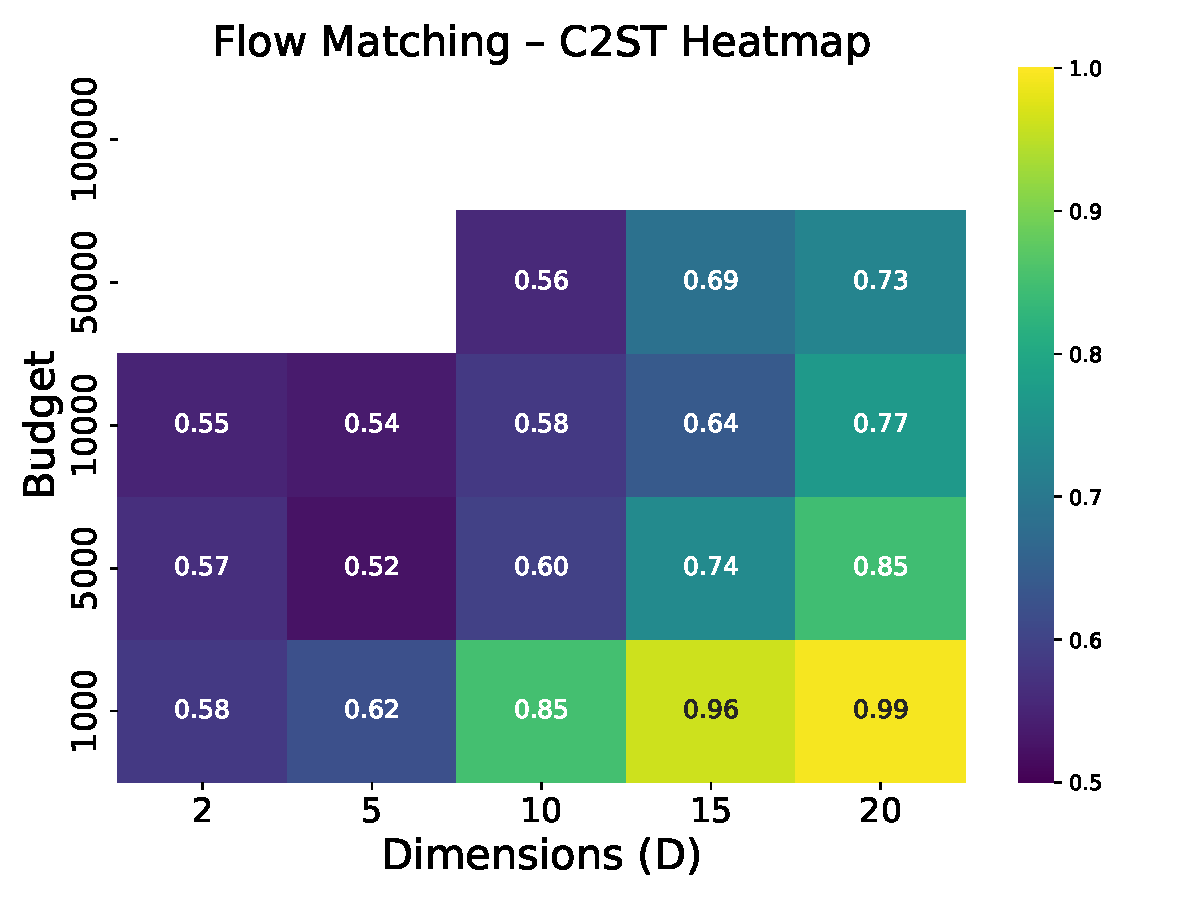
\includegraphics[width=.24\linewidth]{figures/mog_benchmark/single_mode/Flow_Matching_c2st_heatmap}
    \caption{MoG Benchmark - Base simulator: C2ST heatmaps for R2OMC, NPE, BayesFlow, and Flow Matching.}
    \label{fig:mog_benchmark_base_heatmaps}
\end{figure}

\begin{figure}
    \centering
    
\includegraphics[width=.24\linewidth]{figures/mog_benchmark/single_mode_distractors/R2OMC_c2st_heatmap}
    
\includegraphics[width=.24\linewidth]{figures/mog_benchmark/single_mode_distractors/NPE_c2st_heatmap}
    
\includegraphics[width=.24\linewidth]{figures/mog_benchmark/single_mode_distractors/BayesFlow_c2st_heatmap}
    
\includegraphics[width=.24\linewidth]{figures/mog_benchmark/single_mode_distractors/Flow_Matching_c2st_heatmap}
    \caption{MoG Benchmark - Base simulator with distractors: C2ST heatmaps for R2OMC, NPE, BayesFlow, and Flow Matching.}
    \label{fig:mog_benchmark_base_distractors_heatmaps}
\end{figure}

\begin{figure}
    \centering
    
\includegraphics[width=.24\linewidth]{figures/mog_benchmark/two_modes/R2OMC_c2st_heatmap}
    
\includegraphics[width=.24\linewidth]{figures/mog_benchmark/two_modes/NPE_c2st_heatmap}
    
\includegraphics[width=.24\linewidth]{figures/mog_benchmark/two_modes/BayesFlow_c2st_heatmap}
    
\includegraphics[width=.24\linewidth]{figures/mog_benchmark/two_modes/Flow_Matching_c2st_heatmap}
    \caption{MoG Benchmark - MoG simulator: C2ST heatmaps for R2OMC, NPE, BayesFlow, and Flow Matching.}
    \label{fig:mog_benchmark_mog_heatmaps}
\end{figure}

\begin{figure}
    \centering
    
\includegraphics[width=.24\linewidth]{figures/mog_benchmark/two_modes_distractors/R2OMC_c2st_heatmap}
    
\includegraphics[width=.24\linewidth]{figures/mog_benchmark/two_modes_distractors/NPE_c2st_heatmap}
    
\includegraphics[width=.24\linewidth]{figures/mog_benchmark/two_modes_distractors/BayesFlow_c2st_heatmap}
    
\includegraphics[width=.24\linewidth]{figures/mog_benchmark/two_modes_distractors/Flow_Matching_c2st_heatmap}
    \caption{MoG Benchmark - MoG simulator with distractors: C2ST heatmaps for R2OMC, NPE, BayesFlow, and Flow Matching.}
    \label{fig:mog_benchmark_mog_distractors_heatmaps}
\end{figure}


\subsection{SBI - SLCP (T.3) and SLCP Distractors (T.4)}

We here provide additional information on example T.3 and T.4 of the SBI benchmark~\cite{lueckmann2021benchmarking}.

SLCP (T.3):

\begin{tabular}{@{}ll@{}}
  \textbf{Prior} & $\thb \sim \mathcal{U}(-\mathbf{3}, \mathbf{3})$ \\ [5pt]
  \textbf{Simulator} & $\yb = (\boldsymbol{y_1}, \ldots, \boldsymbol{y_4}), \boldsymbol{y_i} \sim \mathcal{N}(\boldsymbol{m_{\theta}}, \boldsymbol{S_{\theta}}) \in \mathbb{R}^2 $ \\ [5pt]
                 & where: $\boldsymbol{m_{\theta}} \sim \begin{bmatrix}  \theta_1 \\ \theta_2 \end{bmatrix},
                   \boldsymbol{S_{\theta}} = \begin{bmatrix} s_1 & \rho s_1 s_2 \\ \rho s_1 s_2 & s_2^2  \end{bmatrix}$,
                   where $s_1 = \theta_3^2$, $s_2 = \theta_4^2$ and $\rho = \tanh \theta_5$ \\ [10pt]
  \textbf{Dimensionality} & $\thb \in \mathbb{R}^{5}$, $\boldsymbol{y_i} \in \mathbb{R}^{2}$, $\yb \in \mathbb{R}^{8}$ \\ [5pt]
\end{tabular}

SLCP with distractors (T.4):

\begin{tabular}{@{}ll@{}}
  \textbf{Prior} & $\thb \sim \mathcal{U}(-\mathbf{3}, \mathbf{3})$ \\ [5pt]
  \textbf{Simulator} & $\yb = (\boldsymbol{y_1}, \ldots, \boldsymbol{y_4})$, $\boldsymbol{y_i} = (\boldsymbol{y_i^{(0)}}, \boldsymbol{y_i^{(1)}})$ where $\boldsymbol{y_i^{(0)}} \sim \mathcal{N}(\boldsymbol{m_{\theta}}, \boldsymbol{S_{\theta}}) $ \\ [5pt]
                 & where: $\boldsymbol{m_{\theta}} \sim \begin{bmatrix}  \theta_1 \\ \theta_2 \end{bmatrix},
                   \boldsymbol{S_{\theta}} = \begin{bmatrix} s_1 & \rho s_1 s_2 \\ \rho s_1 s_2 & s_2^2  \end{bmatrix}$,
                   $s_1 = \theta_3^2$, $s_2 = \theta_4^2$ and $\rho = \tanh \theta_5$ \\ [10pt]
                 & and $\boldsymbol{y_i^{(1)}}$ comes from a distribution (independent of $\thb$) analyzed in \citep{lueckmann2021benchmarking}. \\ [5pt]
  \textbf{Dimensionality} & $\thb \in \mathbb{R}^{5}$, $\boldsymbol{y_i} \in \mathbb{R}^{100}$, $\boldsymbol{y_i} \in \mathbb{R}^{25}$, $\boldsymbol{y_i^{(0)}} \in \mathbb{R}^{2}$, $\boldsymbol{y_i^{(0)}} \in \mathbb{R}^{23}$ \\ [5pt]
\end{tabular}

The ground truth posterior is not available in closed form. Instead a set of $10{,}000$ posterior samples is used


\subsubsection{Experimental Setup and Results}

We evaluate \rromc~using simulation budgets (i.e., numbers of seeds) of 1{,}000, 1{,}500, 5{,}000, 10{,}000, and 30{,}000. 
The SBI benchmark provides 10{,}000 ground-truth posterior samples for each of eight distinct observations. 
We run \rromc~on all observations and report the mean \CtwoST~score and mean runtime across them.

Figure~\ref{fig:slcp_c2st_runtime} in the main paper presents the \CtwoST--runtime plots for both T.3 and T.4 tasks. 
To complement these, Figure~\ref{fig:exp_sbi_slcp} shows the \CtwoST--budget and runtime--budget relationships for the same tasks. 
These results confirm that the increase in runtime is primarily driven by the larger simulation budgets required for accurate inference.

Figure~\ref{fig:slcp_posterior} in the main paper illustrates how \rromc~handles multiple observations. 
Proposal samples are first selected per observation (within an $\epsilon$-distance) and then reweighted according to Eq.~\ref{eq:rromc_weight} to retain those most consistent across all observations. 
In Figure~\ref{fig:exp_sbi_slcp_samples}, we visualize all proposal samples from all observations (left panel), the subset that receives positive weights (middle panel), and the final accepted samples (right panel).

Overall, results demonstrate that \rromc~accurately approximates the posterior, achieving mean \CtwoST~scores in the range of 0.7--0.8 within only a few seconds. 
In contrast, competing methods require substantially higher budgets (typically $10^4$--$10^5$ simulations) and correspondingly longer runtimes—often several hours—to reach comparable performance. 
The performance gap becomes particularly pronounced in distractor settings, where most competing methods fail to achieve \CtwoST~scores below 0.8 regardless of the simulation budget.


\begin{figure}
\centering
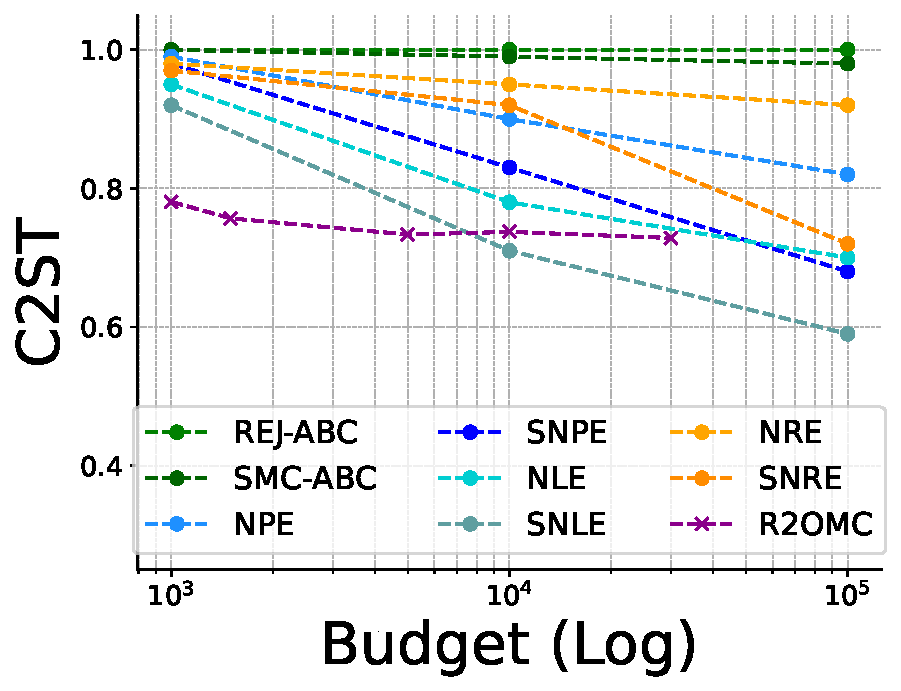
\includegraphics[width=.24\linewidth]{figures/sbibm/slcp/c2st}
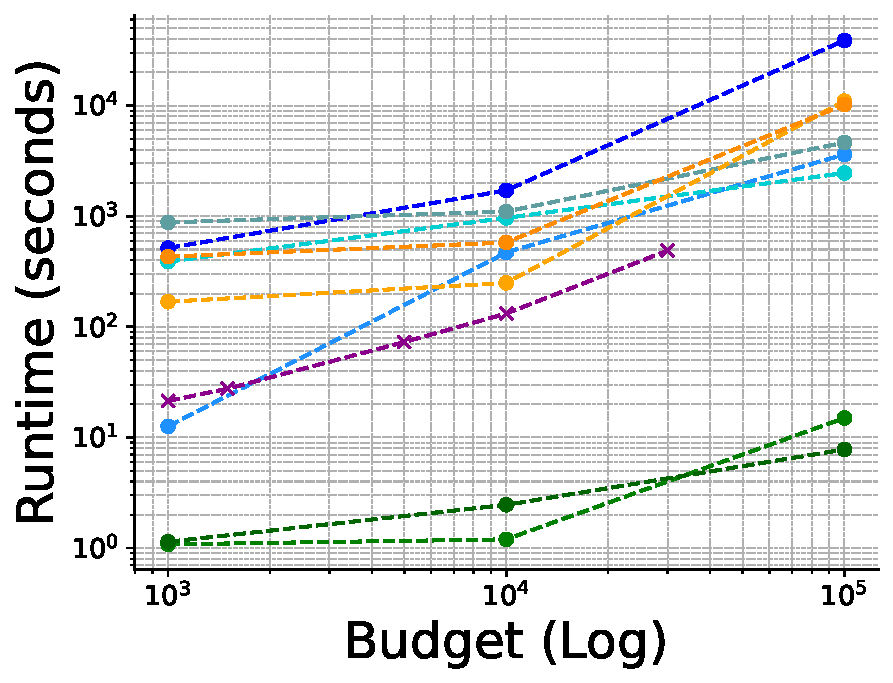
\includegraphics[width=.24\linewidth]{figures/sbibm/slcp/runtime}

\includegraphics[width=.24\linewidth]{figures/sbibm/slcp_distractors/c2st}

\includegraphics[width=.24\linewidth]{figures/sbibm/slcp_distractors/runtime}
\caption{From left to right: \texttt{C2ST} vs. budget, runtime vs. budget. for T.3: SLCP and same figures for (T.4: SLCP Distractors)}
\label{fig:exp_sbi_slcp}
\end{figure}


\begin{figure}
    \centering
    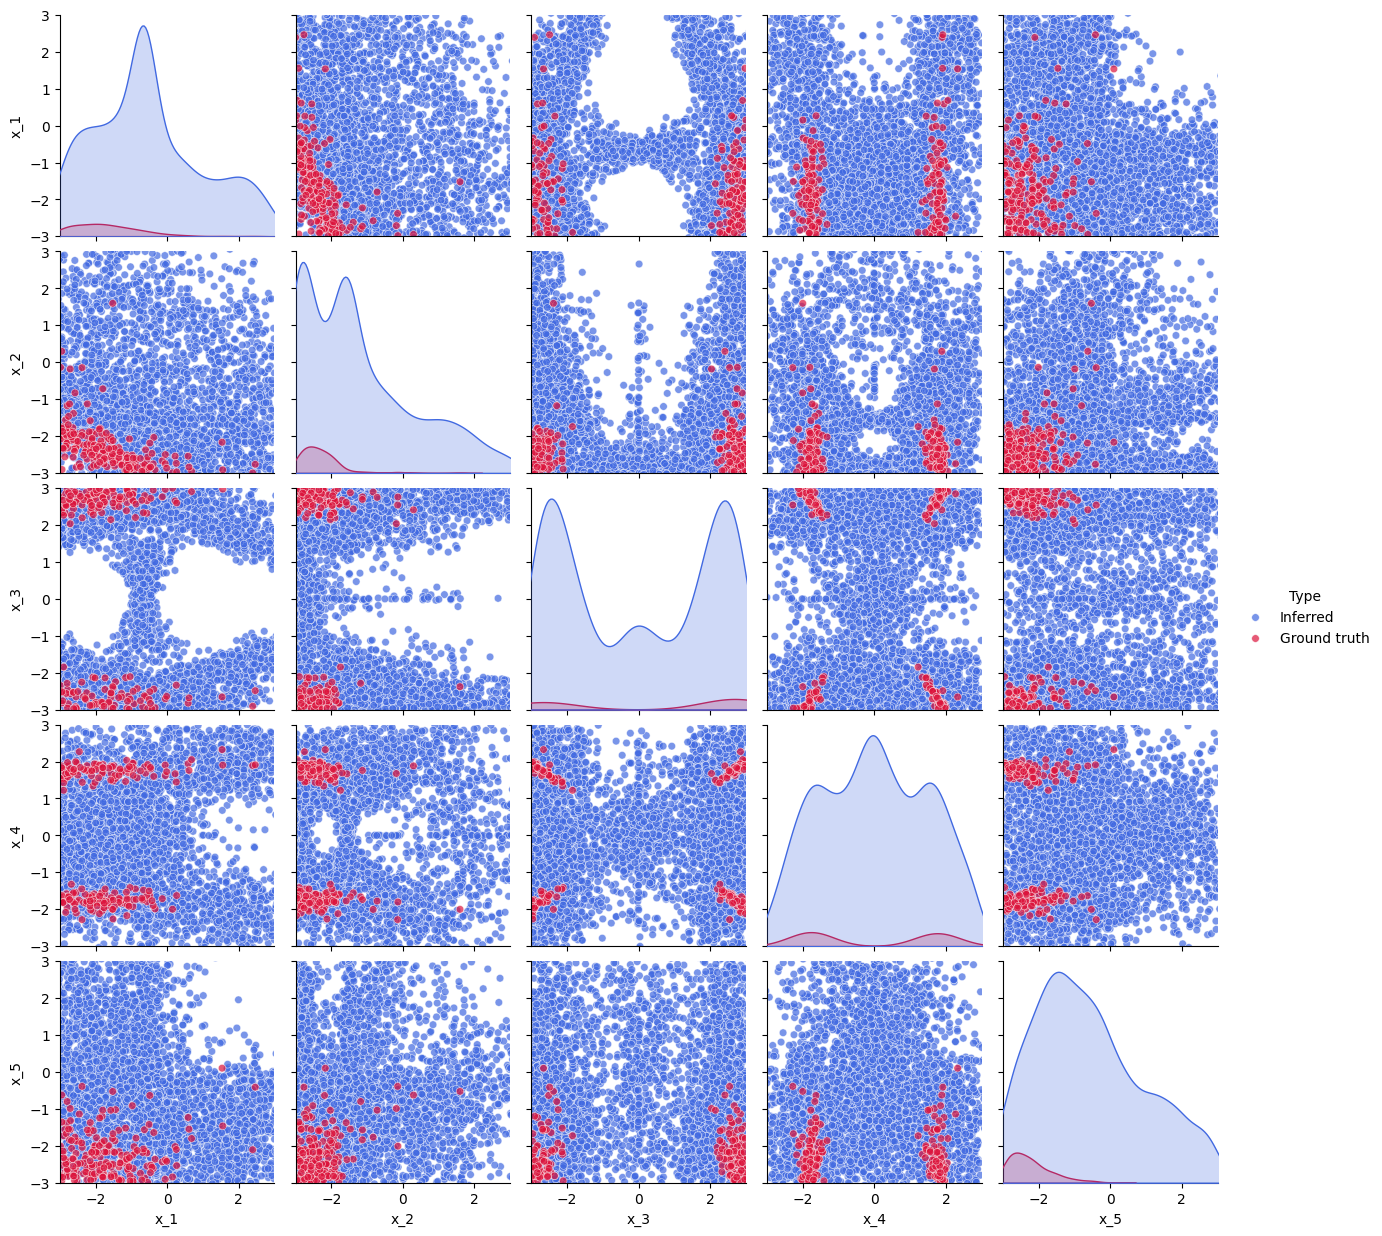
\includegraphics[width=.32\linewidth]{./figures/sbibm/slcp/pairwise_posterior_total}
    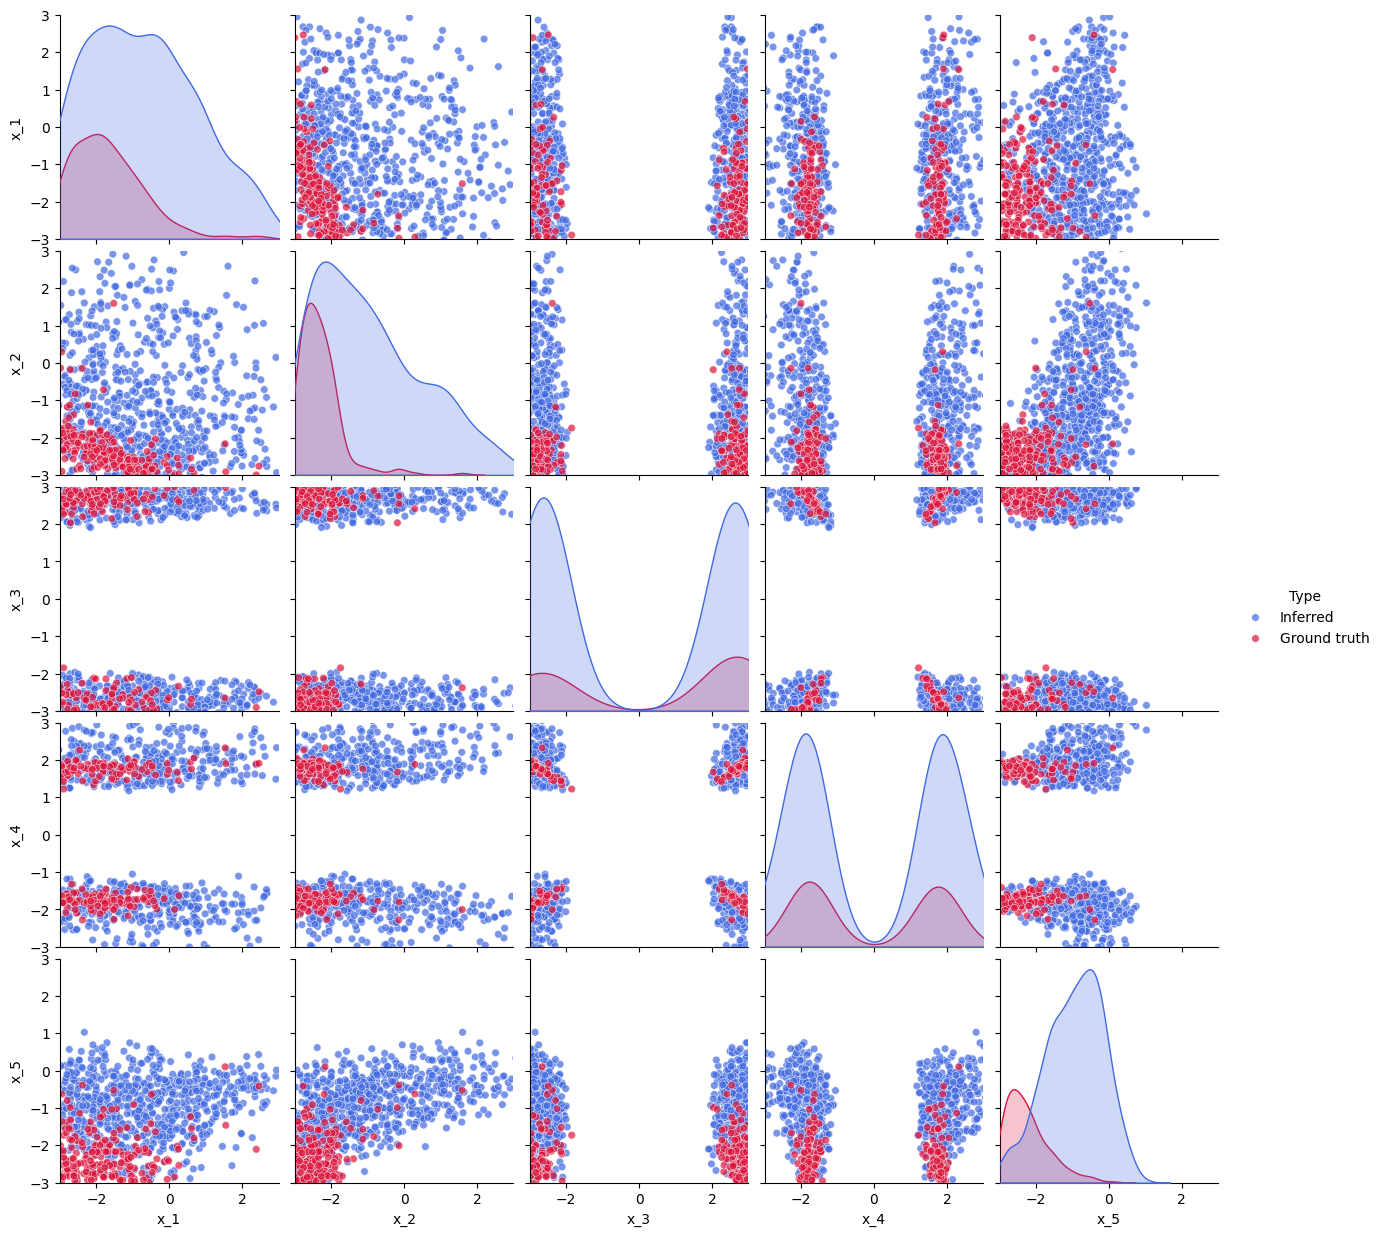
\includegraphics[width=.32\linewidth]{./figures/sbibm/slcp/pairwise_posterior_accepted}
    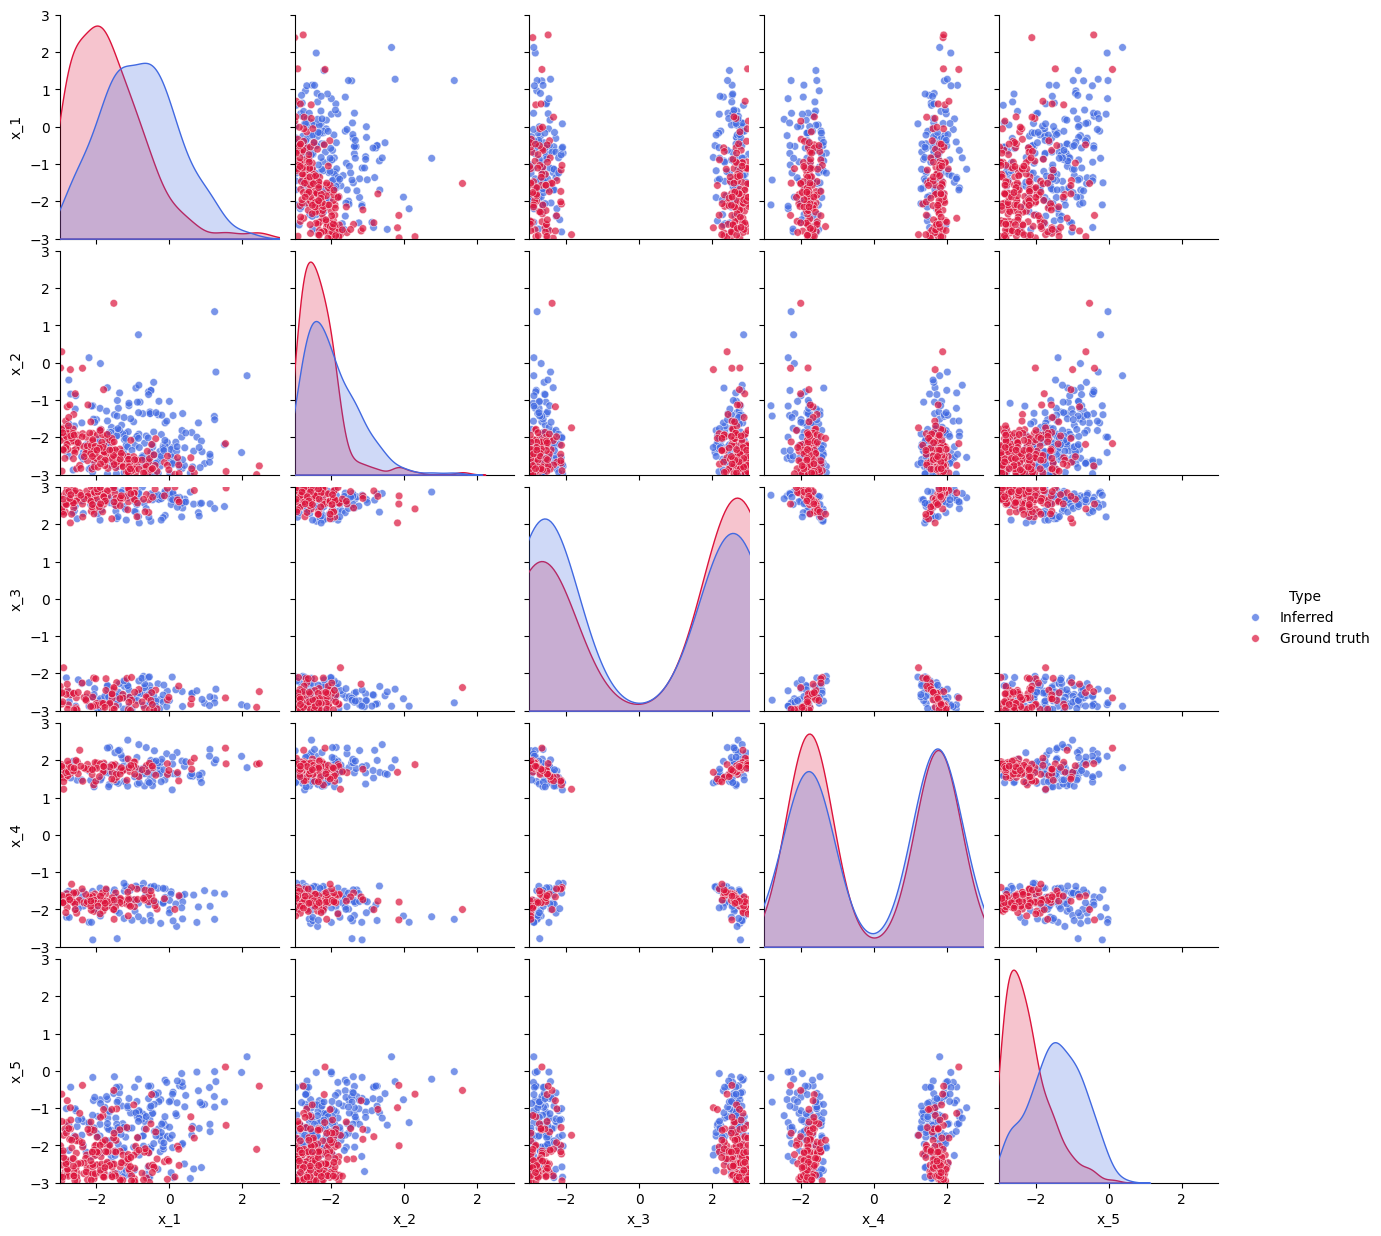
\includegraphics[width=.32\linewidth]{./figures/sbibm/slcp/pairwise_posterior_selected}
    \caption{T.3: SLCP. From left to right: total samples, accepted samples, and selected samples by R2OMC.}
    \label{fig:exp_sbi_slcp_samples}
\end{figure}


\subsection{SBI - Two Moons (T.8)}

We here provide additional information on example T.8 of the SBI benchmark~\cite{lueckmann2021benchmarking}.
It tests inference when the posterior exhibits both global (bimodality) and local (crescent shape) structure to illustrate how algorithms deal with multimodality:

\begin{tabular}{@{}ll@{}}
  \textbf{Prior} & $\thb \sim \mathcal{U}(-\mathbf{1}, \mathbf{1})$ \\ [5pt]
  \textbf{Simulator} & $\yb \sim \begin{bmatrix} 
    r \cos(\alpha) + 0.25 \\ 
    r \sin(\alpha)
  \end{bmatrix} + \begin{bmatrix} 
    |\theta_1 + \theta_2|/\sqrt{2} \\ 
    (-\theta_1 + \theta_2)/\sqrt{2}
  \end{bmatrix}$, where $r \sim \mathcal{N}(0.1, 0.01^2)$ and $\alpha \sim \mathcal{U}(-\pi/2, \pi/2)$ \\ [10pt]
  \textbf{Dimensionality} & $\thb \in \mathbb{R}^{2}$, $\yb \in \mathbb{R}^{2}$ \\ [5pt]
\end{tabular}

The ground truth posterior is not available in closed form. Instead a set of $10{,}000$ posterior samples is used

\subsubsection{Experimental Setup and Results}

We test ROMC for simulation budget (number of seeds) equal to 1000, 5000, 10000.
SBI benchamrk provides a set of 10{,}000 gound-truth posterior samples for each of the 8 different observations.
We run ROMC in all observations and we report the mean C2ST score and the mean runtime across themm.
Figure~\ref{fig:sbi_two_moons} in the main paper shows the C2ST vs. runtime plot and the pairwise posterior plot.
To compliment that, in Figure~\ref{fig:exp_sbi_two_moons} we provide the C2T vs. budget plot and the Budget vs. Rutime.
These plot confirm that the reason behind higher duntimes is the increase in the budget. 

\rromc~achieves a near-optimal \CtwoST score ($\approx 0.5$) in a few-seconds runtime as 1000 different seeds $S$ are already enough for a good posterior approximaiont.
Competing methods require minutes to hours (budgets of $10^5$ samples) to reach comparable performance (which never becomes that good)
The pairwise posterior further demonstrates that \rromc~accurately captures both crescent-shaped modes.


\begin{figure}[ht]
  \centering
  \begin{subfigure}[b]{0.45\linewidth}
    \centering
    
\includegraphics[width=\linewidth]{figures/sbibm/two_moons/c2st}
    \caption{\texttt{C2ST} score}
  \end{subfigure}
  \hfill
  \begin{subfigure}[b]{0.45\linewidth}
    \centering
    
\includegraphics[width=\linewidth]{figures/sbibm/two_moons/runtime}
    \caption{Ground truth samples}
  \end{subfigure}
  \caption{T.8: Two Moons. From left to right: \texttt{C2ST} score, ground truth samples, and samples by R2OMC.}
  \label{fig:exp_sbi_two_moons}
\end{figure}

\clearpage
